\documentclass[journal]{IEEEtran}

\usepackage{cite}

\usepackage{amsmath,amssymb,amsfonts}
\usepackage{algorithm}
\usepackage{graphicx}
\usepackage{textcomp}
\usepackage{xcolor}
\usepackage{booktabs}
\usepackage{multirow}
\usepackage{array}
\usepackage{subfig}
\usepackage{geometry}
%\usepackage{algorithm}
%\usepackage{algpseudocode}
\usepackage{algpseudocode}

\algrenewcommand\algorithmicrequire{\textbf{Input:}}
\algrenewcommand\algorithmicensure{\textbf{Output:}}


\def\BibTeX{{\rm B\kern-.05em{\sc i\kern-.025em b}\kern-.08em
    T\kern-.1667em\lower.7ex\hbox{E}\kern-.125emX}}

\begin{document}

\title{Distributed Collapsed Gibbs Sampling for LDA on Spark}

\author{\IEEEauthorblockN{Agnieszka Ciborowska}\\
\IEEEauthorblockA{\textit{Department of Computer Science} \\
\textit{Virginia Commonwealth University}}}


\maketitle

\begin{abstract}
The report describes a collapsed Gibbs sampling method for widely-used latent Dirichlet allocation (LDA) model on Spark.
\end{abstract}


\begin{IEEEkeywords}
Spark, LDA, collapsed Gibbs sampling
\end{IEEEkeywords}


\section{Introduction}
Processing very large datasets has became a rapidly growing interest of researches as it provides ability for richer analysis

The latent Dirichlet allocation model, proposed by Blei et al.~\cite{blei2003latent}, is a three-level hierarchical Bayesian model designed to discover latent topics in document corpora. The main idea of the model is to represent each document as a random mixture of topics, where each topic is, in turn, modeled by a distribution over words. 

To summarize, the contributions of this report are:
\begin{itemize}
\item implementation of a collapsed Gibbs sampling for LDA on Spark,
\item evaluation of the effectiveness of the Spark-LDA in latent topic discovery,
\item evaluation of the influence of Spark-LDA's parameters on the model performance and execution time.
\end{itemize}
The organization of this report is as follows. Section \ref{sec:lda} contains a brief review of the plain LDA model and collapsed Gibbs sampling procedure, while Section~\ref{sec:slda} provides a detailed description on the distributed LDA implementation using Spark. In Section~\ref{sec:exp}, the report provides the evaluation results compared to the standard LDA. Finally, Section~\ref{sec:conclusion} conclude the report and outlines plan for future work.

\section{Latent Dirichlet Allocation}
\label{sec:lda}
Before describing the details of the distributed LDA model, I briefly review the standard LDA model, presented in Figure~\ref{fig:lda} using a plate notation.  LDA models each of $D$ documents as a mixture over $K$ latent topics, where each topic is a multinomial probability distribution over a vocabulary of $V$ words. Generative process of creating a new document $j$ can be characterized as follows:
\begin{itemize}
\item draw a mixing proportion $\theta_{k|j}$ from a Dirichlet with parameter $\alpha$,
\item for the $i^{th}$ word in the document, first draw a topic assignment $z_{ij}$, where topic $k$ is chosen with probability of $\theta_{k|j}$, and then value $w$ of word $x_{ij}$ is drawn from the $z_{ij}$ topic with probability $\phi_{w|k}$, where $\phi_{w|z_{ij}}$ is drown from a Dirichlet prior with parameter $\beta$.
\end{itemize}
The above description of the generative process is equivalent to:
$$
\theta_{k|j}\sim Dir(\alpha) \quad \phi_{w|k}\sim Dir(\beta)
$$
$$z_{ij}\sim \theta_{k|j} \quad  x_{ij}\sim \phi_{w|z_{ij}}
$$
where $\alpha$ and $\beta$ are fixed Dirichlet priors.

\begin{figure}
\centering
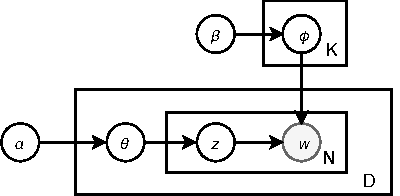
\includegraphics[scale=0.9]{plots/LDA.pdf}
\caption{Graphical model for LDA. Observed variable $w$ is shaded.}
\label{fig:lda}
\end{figure}

Given the observed words $\texttt{x}=x_{\{ij\}}$, the task is to compute the posterior distribution over the latent variables $\texttt{z}$, $\theta$ and $\phi$. The two most frequently used approximate inference procedures are based on either using variational methods\cite{blei2003latent} or Markov chain Monte Carlo (MCMC) methods \cite{griffiths2004finding}. This report focuses on the later, more specifically, on a collapsed Gibbs sampling inference procedure for LDA, proposed by Griffiths and Steyvers\cite{griffiths2004finding}. The collapsed Gibbs sampling samples the latent variable $\texttt{z}$ with $\theta$ and $\phi$ integrated out. In this setup the conditional probability of $z_{ij}$ is given by:
$$
p(z_{ij}=k|z^{\lnot ij}, x, \alpha, \beta) = \dfrac{c_{k,m,\cdot} + \alpha}{N_{j}^{\lnot i}+K\alpha} \frac{c_{k,\cdot,n} + \beta}{c_{k,\cdot,\cdot} + V\beta}
$$ 
where $\lnot ij$ denotes word $i$ in document $j$ that is excluded in the count values and $c_{k,m,n}$ represents the number of times topic $k$ is assigned to word $n$ in document $m$. Missing index value for $c_{k,m,n}$ (e.g. $c_{k,\cdot,n}$) denotes summing over that index (e.g. $c_{k,\cdot,n} = \sum_{m=1}^{M} c_{k,m,n}$).

Implementation of a sequential collapsed Gibbs sampler for LDA is straightforward as it operates on a set of count values, $c_{k,\cdot,m}$, $c_{k,m,\cdot}$ and $c_{k,\cdot,\cdot}$. The algorithm starts by randomly assigning a topic to a word in a document, updating the count values accordingly, and performs loop over the number of iterations to reassign a topic to a word in a according to the conditional probability. The outline of LDA collapsed Gibbs sampling is presented as Algorithm \ref{alg}.
 \begin{algorithm}
\caption{LDA with collapsed Gibbs sampling}
\label{alg}
\begin{algorithmic}
\scriptsize
\Require set of $D$ documents
\Ensure topics assignments $\textbf{z}$ and the count values $c_{k,m,\cdot}$, $c_{k,\cdot,n}$, $c_{k,\cdot,\cdot}$
\State \textbf{begin}
\State randomly initialize $\textbf{z}$ and increment the count values
   \ForAll  {$i = 0 \rightarrow iterations - 1$}
      \ForAll  {$d$ in $D$}
         \ForAll  {$word$ in $d$}
            \State $ topic \rightarrow z[d, word]$
            \State $c_{topic,d,\cdot} -= 1$
            \State $c_{topic,\cdot,word}-=1$
            \State $c_{topic,\cdot,\cdot}-=1$
            \ForAll {$k = 0 \rightarrow K-1$}
            	\State $p(z_{word,d}=k|\cdot) = \dfrac{c_{k,d,\cdot} + \alpha}{N_{d}^{\lnot i}+K\alpha} \frac{c_{k,\cdot,word} + \beta}{c_{k,\cdot,\cdot} + V\beta}$
            \EndFor
            \State $topic \leftarrow$ sample from $p(z|\cdot)$
            \State $z[d, word] \leftarrow topic $
            \State $c_{topic,d,\cdot} += 1$
            \State $c_{topic,\cdot,word} +=1$
            \State $c_{topic,\cdot,\cdot}+=1$
		 \EndFor            
      \EndFor 
   \EndFor
\State \textbf{end}
        \end{algorithmic}
    \end{algorithm}

\section{Distributed inference for LDA}
\label{sec:slda}
Although LDA with collapsed Gibbs sampling has been in common use, due to its high computational complexity, this method it not applicable for processing large document corpora. Additionally, obtaining the speedup through paralellization is not trivial as collapsed Gibbs sampling is a strictly sequential process that uses the current state of all but one variable to sample new topic assignment $z_{ij}$. To distribute the computations, this study follows the approach proposed by Newman et al.\cite{newman2009distributed} and assumes that since number of words in a document is typically larger than number of cores, the dependency between topic assignment $z_{ij}$ and $z_{i'j'}$ is weak, thus the sequential sampling requirement can be relaxed and the LDA model can be trained and tested in a distributed environment.

\subsection{Approximate LDA on Spark}

 \begin{algorithm}
\caption{Distributed LDA with collapsed Gibbs sampling}
\label{alg2}
\begin{algorithmic}
\scriptsize
\State \textbf{begin}
\State randomly initialize $\textbf{z}$ and increment the count values
\State update global counts $c_{k,\cdot,n}$, $c_{k,\cdot,\cdot}$
\State divide $D$ documents into $p$ partitions
 \ForAll  {$i = 0 \rightarrow iterations - 1$}
   \ForAll  {partition $p$ in parallel}
   	  \State copy global counts $c_{k,\cdot,n}$, $c_{k,\cdot,\cdot}$
   	  \State perform LDA($D_p$)
   \EndFor
   \State update global counts $c_{k,\cdot,n}$, $c_{k,\cdot,\cdot}$
  \EndFor
\State \textbf{end}
\end{algorithmic}
\end{algorithm}


\section{Experiments}
\label{sec:exp}




\begin{figure*}[t]
\centering
\subfloat[ABC news headlines dataset.]{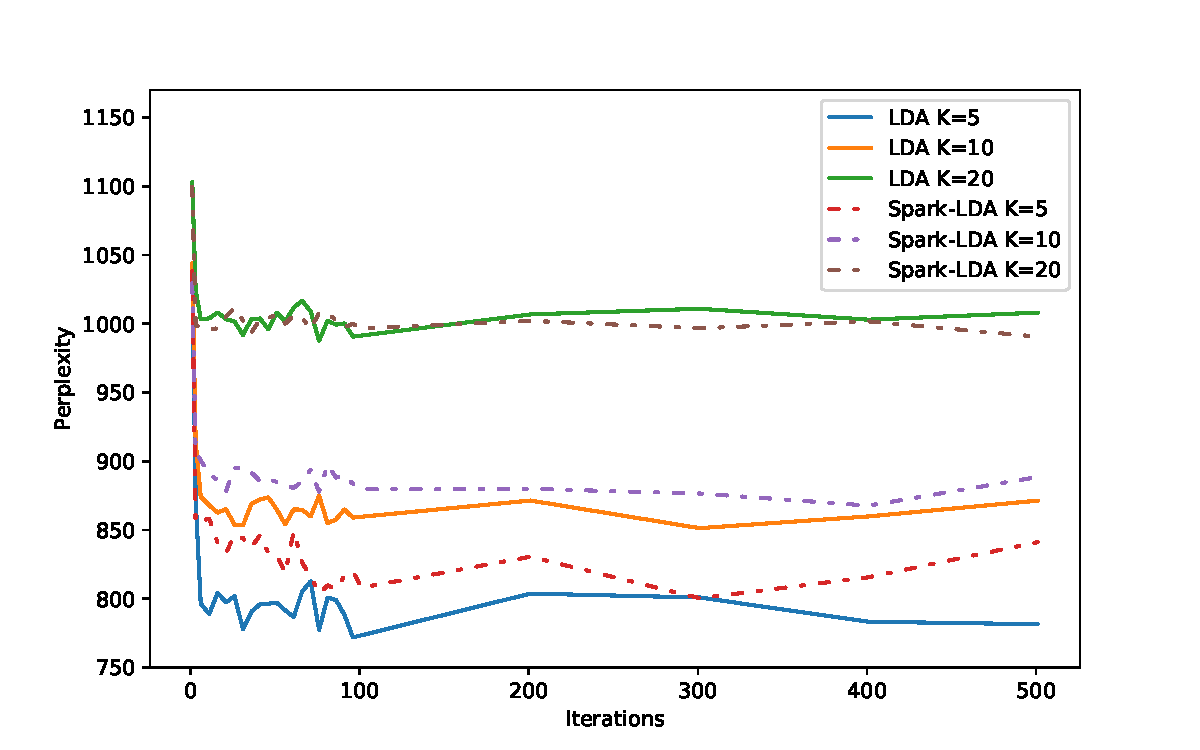
\includegraphics[scale=0.44]{plots/perplexity1.pdf}%
\label{fig:perplex2}}
\hfil
\subfloat[NIPS abstracts dataset.]{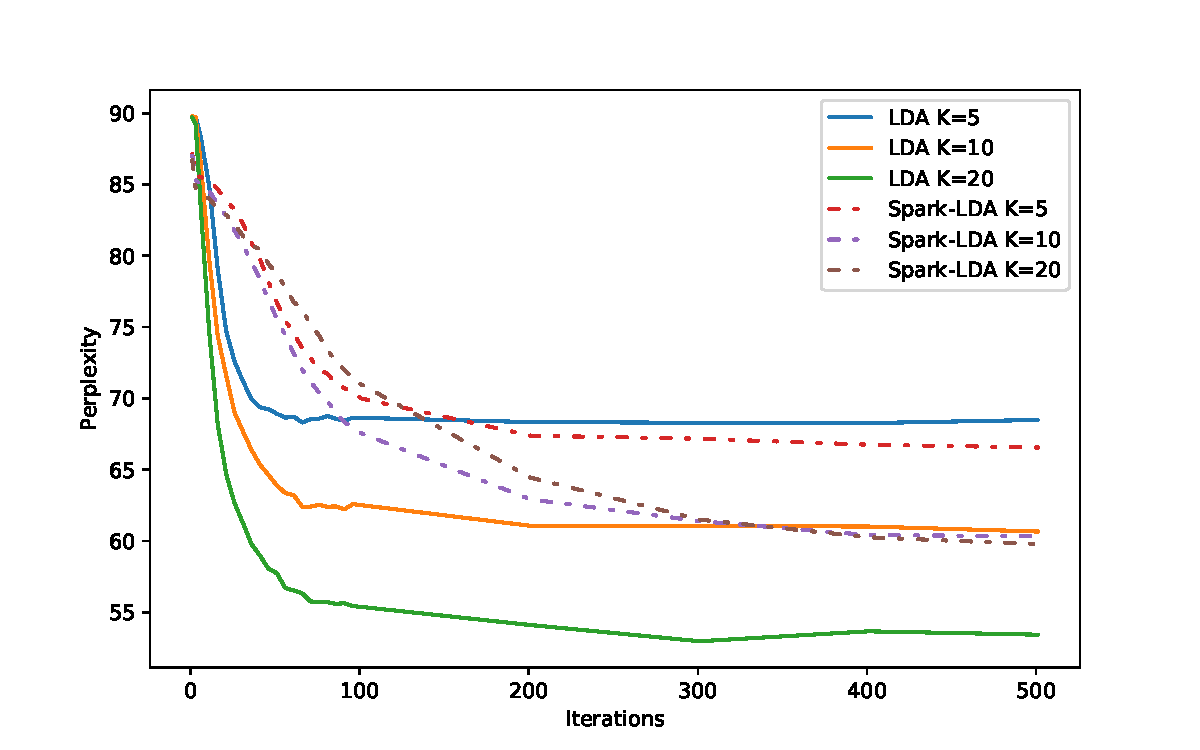
\includegraphics[scale=0.44]{plots/perplexity2.pdf}%
\label{fig:perplex2}}
\caption{Perplexity during training for different number of topics.}
\label{fig_sim}
\end{figure*}

\renewcommand{\arraystretch}{1.3}

\begin{table*}[t]
\centering
\caption{Execution time in seconds and speedup achieved by Spark-LDA with respect to different number of topics.}
\begin{tabular}{lrrrrrrr} \toprule
                 & \multicolumn{3}{c}{\textbf{ABC News headlines}} & \multicolumn{3}{c}{\textbf{NIPS abstracts}}        & \multicolumn{1}{c}{\textbf{ABC News headlines (full)}} \\
                 & K = 5             & K = 10           & K = 20           & K = 5           & K = 10          & K = 20         & K = 2                                           \\ \midrule
LDA              & 47,80             & 51,59            & 57,41            & 1 729,06        & 1 779,65        & 2 002,13       & 32 577,60                                       \\
Spark-LDA        & 117,27            & 126,82           & 143,06           & 128,03          & 159,32          & 207,01         & 3 929,08                                        \\ \midrule
\textbf{Speedup} & \textbf{0,408}    & \textbf{0,407}   & \textbf{0,401}   & \textbf{13,505} & \textbf{11,170} & \textbf{9,672} & \textbf{8,291}  \\ \bottomrule                         
\end{tabular}
\label{tab:speedup}
\end{table*}

\begin{figure*}[t]
\centering
\subfloat[ABC News headlines dataset.]{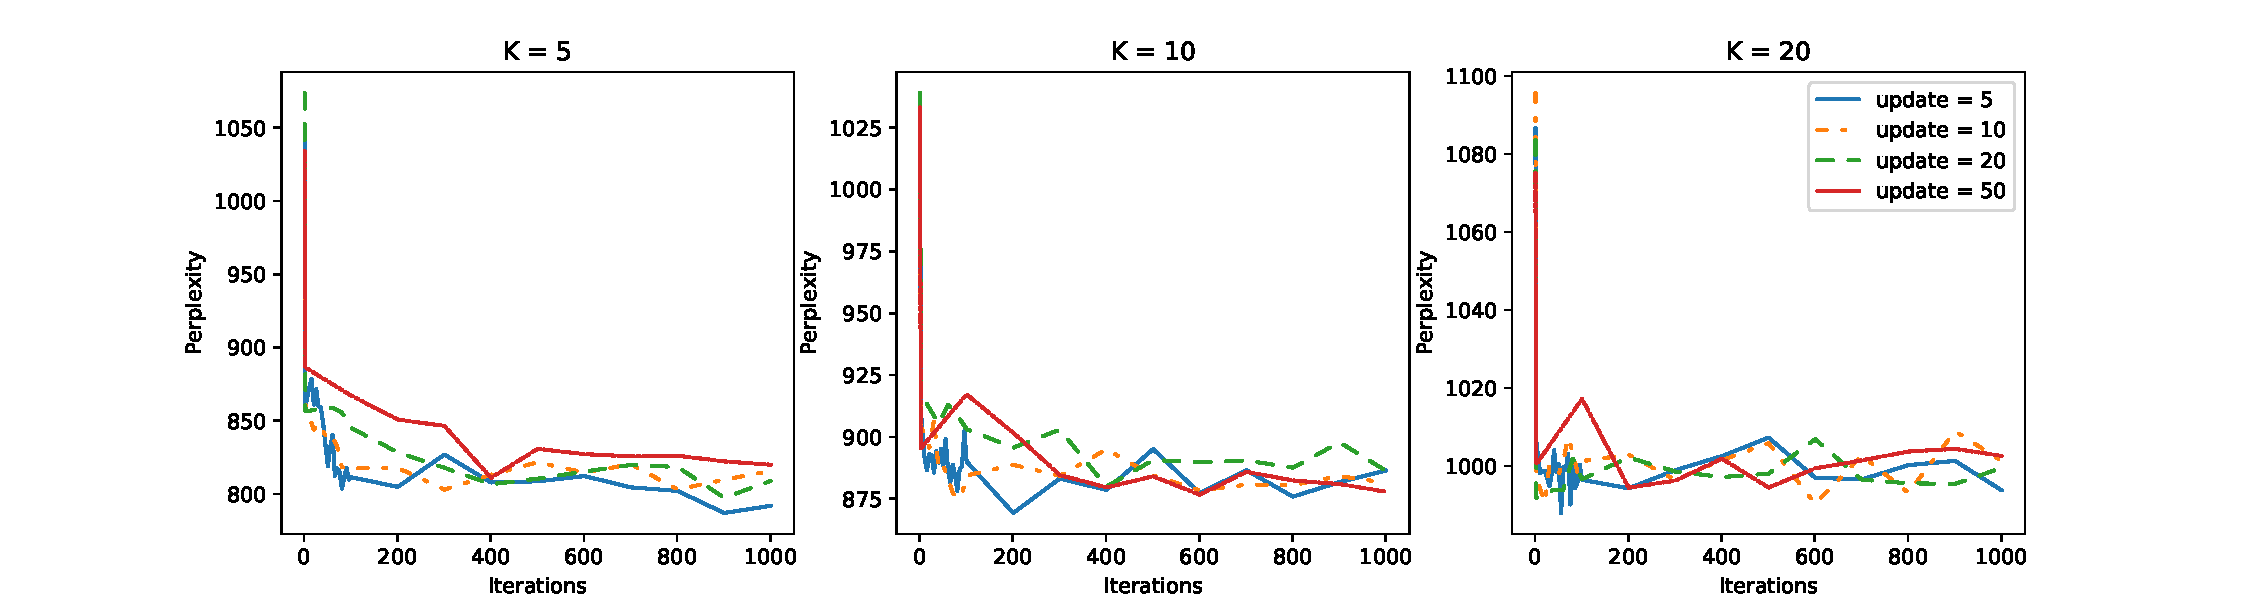
\includegraphics[scale=0.5]{plots/update_abc.pdf}%
\label{fig:param_abc}}
\hfil
\subfloat[NIPS abstracts dataset.]{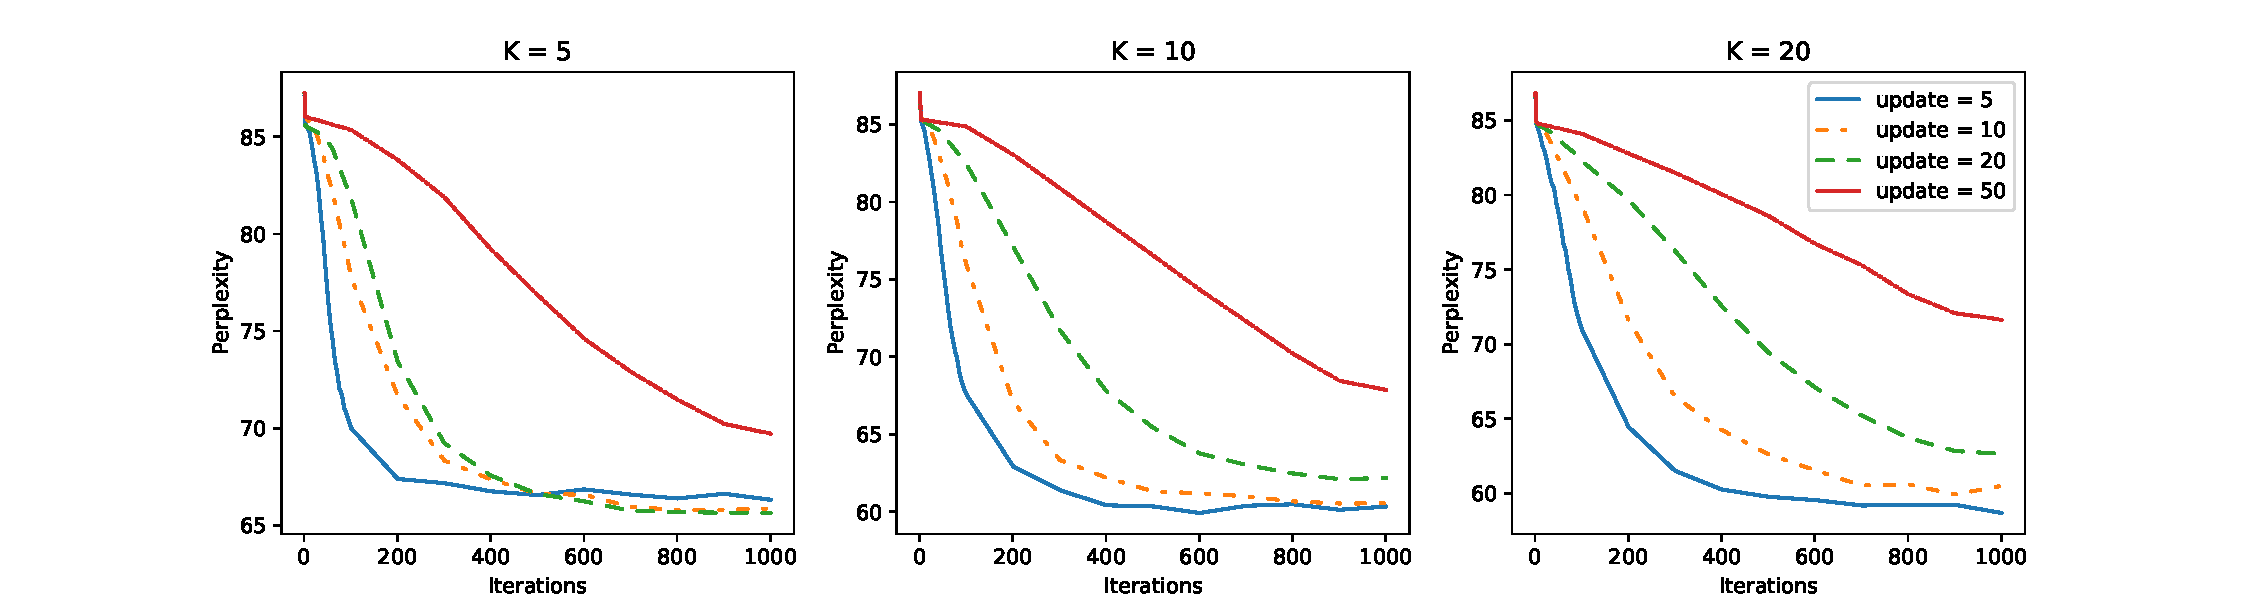
\includegraphics[scale=0.5]{plots/update_abstract.pdf}%
\label{fig:param_nips}}
\caption{Perplexity during training Spark-LDA for different interval between parameter updates .}
\label{fig_sim}
\end{figure*}

\begin{figure*}[t]
\centering
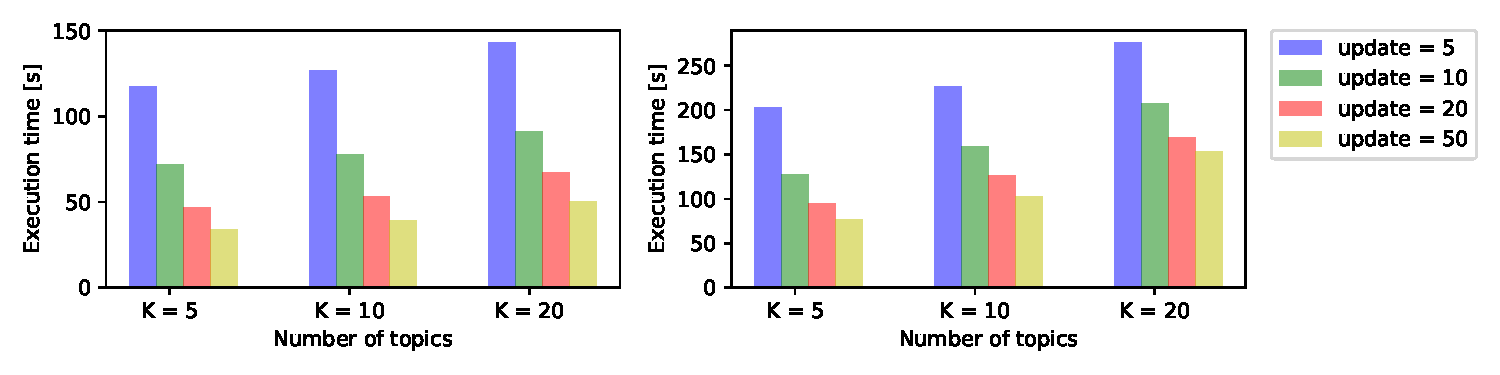
\includegraphics[scale=0.7]{plots/param_update.pdf}
\caption{Execution time of Spark-LDA on ABC News headlines (left) and NIPS abstracts (right) with respect to interval between global parameters update.}
\label{fig_sim}
\end{figure*}



\section{Conclusion}
\label{sec:conclusion}


\bibliographystyle{IEEEtran}
\bibliography{IEEEabrv,paper}


\end{document}


